\documentclass[12pt, a4paper]{report}

% =================================================================
% 1. PACKAGES & TYPOGRAPHY setup
% =================================================================
\usepackage[utf8]{inputenc}
\usepackage{mathptmx}           % Times New Roman for Text AND Math (Guideline 6.1)
\usepackage[T1]{fontenc}        % Better font encoding
\usepackage{graphicx}           % For images
\usepackage{geometry}           % Page margins
\usepackage{setspace}           % Line spacing
\usepackage{titlesec}           % Heading formatting
\usepackage{tocloft}            % TOC formatting
\usepackage{amsmath}            % Math formulas
\usepackage{amssymb}            % Math symbols
\usepackage[numbers]{natbib}    % References (BibTeX + natbib) - numeric, square-style citations
\usepackage{caption}            % Caption formatting
\usepackage{array}              % Table formatting
\usepackage{booktabs}           % Professional tables (IEEE Style)
\usepackage{float}              % Figure positioning
\usepackage{fancyhdr}           % Page numbering
\usepackage{listings}           % For code snippets
\usepackage{xcolor}             % For code coloring
\usepackage{url}                % For URLs
\usepackage{microtype}          % Improved typography
\usepackage{multirow}           % For complex tables
\usepackage{tikz}
\usetikzlibrary{arrows.meta, positioning, decorations.pathreplacing}
\usepackage{colortbl}

% \usepackage[none]{hyphenat}

% Ensure consistent Times font family for text and math
\renewcommand{\rmdefault}{ptm}
\normalfont

% Useful cross-reference packages (hyperref last)
\usepackage{cleveref}
\usepackage[hidelinks]{hyperref}

% =================================================================
% 2. PAGE LAYOUT & MARGINS (Guideline 4)
% =================================================================
\geometry{
    a4paper,
    top=35mm,       % Guideline: 30-35mm
    left=40mm,      % Guideline: 35-40mm
    bottom=30mm,    % Guideline: 25-30mm
    right=25mm      % Guideline: 20-25mm
}

% =================================================================
% 3. HEADING FORMATTING (Guideline 5 & 6)
% =================================================================

% Chapter Headings: Centered, All Caps, 50mm from top edge
% Calculation: Top Margin (35mm) + Spacing (15mm) = 50mm visual drop.
\titleformat{\chapter}[display]
  {\normalfont\bfseries\centering}
  {\MakeUppercase{\chaptertitlename}\ \thechapter}{14pt}{\Large\MakeUppercase}
\titlespacing*{\chapter}{0pt}{15mm}{2\baselineskip}

% Section Headings: Left aligned, All Caps, Bold (Guideline 5)
\titleformat{\section}
  {\normalfont\bfseries\large}
  {\thesection}{1em}{\MakeUppercase}
\titlespacing*{\section}{0pt}{1.5\baselineskip}{1\baselineskip}

% Subsection Headings: Left aligned, Sentence Case, Bold (Guideline 5)
\titleformat{\subsection}
  {\normalfont\bfseries\normalsize}
  {\thesubsection}{1em}{}
\titlespacing*{\subsection}{0pt}{1.5\baselineskip}{1\baselineskip}

% Paragraph Indentation (Guideline 6.1)
\setlength{\parindent}{15mm}

% =================================================================
% 4. HEADER & FOOTER (Guideline 7.1)
% =================================================================
\pagestyle{fancy}
\fancyhf{}
\fancyhead[R]{\thepage}     % Page number top right, 20mm from top
\renewcommand{\headrulewidth}{0pt}
\setlength{\headheight}{15pt}

% =================================================================
% 5. CAPTION & CODE STYLING
% =================================================================
\captionsetup[table]{name=Table, labelfont=bf, labelsep=colon, position=top}
\captionsetup[figure]{name=Fig., labelfont=bf, labelsep=colon, position=bottom}

\lstset{
    basicstyle=\ttfamily\small,
    breaklines=true,
    frame=single,
    backgroundcolor=\color{gray!5},
    keywordstyle=\color{blue},
    commentstyle=\color{green!40!black},
    stringstyle=\color{red},
    captionpos=b,
    numbers=left,
    numberstyle=\tiny\color{gray},
    numbersep=5pt
}

% =================================================================
% 6. DOCUMENT DATA
% =================================================================
\newcommand{\thesisTitle}{SAGEAUTOFORMER: A SCALABLE SERIES-AWARE FRAMEWORK FOR ULTRA-LONG MULTIVARIATE TIME-SERIES FORECASTING}
\newcommand{\studentName}{AVULA KARTHIK}
\newcommand{\rollNo}{206124008}
\newcommand{\degree}{MASTER OF TECHNOLOGY}
\newcommand{\specialization}{COMPUTER SCIENCE AND ENGINEERING}
\newcommand{\guideName}{Dr. A. SANTHANA VIJAYAN}
\newcommand{\hodName}{Dr. [HOD NAME]}
\newcommand{\deptName}{DEPARTMENT OF COMPUTER SCIENCE AND ENGINEERING}
\newcommand{\instituteName}{NATIONAL INSTITUTE OF TECHNOLOGY}
\newcommand{\instituteAddress}{TIRUCHIRAPPALLI -- 620 015}
\newcommand{\monthYear}{JULY 2025}

% =================================================================
% 7. MAIN DOCUMENT START
% =================================================================
\begin{document}

% -----------------------------------------------------------------
% TITLE PAGE (Appendix 1)  -- REPLACED WITH STABLE SINGLE-PAGE LAYOUT
% -----------------------------------------------------------------
\begin{titlepage}
    \thispagestyle{empty}
    \centering
    \onehalfspacing

    \vspace*{1.2cm}

    {\bfseries\Large
    SAGEAUTOFORMER:\\[4pt]
    A SCALABLE SERIES-AWARE FRAMEWORK\\[4pt]
    FOR ULTRA-LONG MULTIVARIATE\\[4pt]
    TIME-SERIES FORECASTING
    \par}

    \vspace{1.6cm}

    {\small A thesis submitted in partial fulfillment of the requirements\\
    for the award of the degree of}

    \vspace{1.0cm}

    {\bfseries M.Tech}

    \vspace{0.4cm}

    in

    \vspace{0.4cm}

    {\bfseries COMPUTER SCIENCE AND ENGINEERING}

    \vspace{1.3cm}

    By

    \vspace{0.4cm}

    {\bfseries AVULA KARTHIK}\\
    (206124008)

    \vspace{1.6cm}

    % -------------------------
    % Logo: include if file exists, otherwise show framed placeholder
    % -------------------------
    \IfFileExists{logo.png}{%
        \includegraphics[width=2.6cm,height=2.6cm,keepaspectratio]{logo.png}%
    }{%
        \fbox{\parbox[c][2.6cm][c]{2.6cm}{\centering\textbf{LOGO}}}%
    }

    \vspace{0.2 cm}

    {\bfseries
    DEPARTMENT OF COMPUTER SCIENCE AND ENGINEERING\\
    NATIONAL INSTITUTE OF TECHNOLOGY\\
    TIRUCHIRAPPALLI -- 620015
    }

    \vfill % stretches so that the next line stays at bottom of titlepage

    {\bfseries JULY 2025}

\end{titlepage}

% -----------------------------------------------------------------

% -----------------------------------------------------------------
% BONAFIDE CERTIFICATE (Appendix 2 - Double Spacing)
% -----------------------------------------------------------------
\clearpage
\thispagestyle{plain}
\pagenumbering{roman}
\setcounter{page}{2}

\begin{center}
    \vspace*{10mm}
    {\bfseries\large BONAFIDE CERTIFICATE \par}
    \vspace{2\baselineskip}
\end{center}

\doublespacing
This is to certify that the Report on Project Work (Phase II) titled \textbf{\thesisTitle} is a bonafide record of the work done by \textbf{\studentName} (\rollNo), studying in \textbf{\degree} (\textbf{\specialization}) in the \textbf{\instituteName, TIRUCHIRAPPALLI}, during the year 2024-2025.

\vspace{3.5cm}

\noindent
\begin{minipage}[t]{0.45\textwidth}
    \textbf{\guideName} \\
    Guide \\
    \deptName
\end{minipage}
\hfill
\begin{minipage}[t]{0.45\textwidth}
    \raggedleft
    \textbf{Dr. Kunwar Singh} \\
    Head of the Department \\
    \deptName
\end{minipage}

\vspace{2.5cm}
\noindent Project Viva-voce held on ...................................
\vspace{1.5cm}

\noindent
\begin{minipage}[t]{0.45\textwidth}
    INTERNAL EXAMINER
\end{minipage}
\hfill
\begin{minipage}[t]{0.45\textwidth}
    \raggedleft
    EXTERNAL EXAMINER
\end{minipage}

% -----------------------------------------------------------------
% ABSTRACT (Guideline 5.3)
% -----------------------------------------------------------------
\clearpage
\begin{center}
    \vspace*{10mm}
    {\bfseries\LARGE ABSTRACT \par}
    \vspace{4\baselineskip}
\end{center}
\onehalfspacing

Long-term multivariate time-series forecasting aims to predict several related variables over extended horizons and is important for domains such as traffic control, power load planning, and climate monitoring. The core difficulty comes from the need to model both within-series temporal patterns (e.g., trends and seasonality) and cross-series dependencies that arise from the underlying system connections.

Recent architectures like SageFormer combine Graph Neural Networks (GNNs) to model inter-variable relations and Transformer-like temporal modules to model time dependencies \citep{Zhang2024}. However, the typical dense self-attention used for temporal modeling scales quadratically with the input length: computing the pairwise query–key interactions produces an $L\times L$ matrix, so runtime and memory grow as $\mathcal{O}(L^2)$ \citep{Vaswani2017}. This growth limits the practical look-back window on standard GPUs and leads to out-of-memory failures when $L$ becomes large.

This work proposes \textbf{SageAutoformer}, which retains series-aware spatial modeling while replacing dense attention with an FFT-based auto-correlation mechanism to lower the temporal cost to approximately $\mathcal{O}(L\log L)$ \citep{Wu2021}. We also apply explicit series decomposition to separate trend and seasonal parts, which helps the model remain stable under non-stationary conditions.

On the Traffic dataset (862 sensors), experiments show the expected trade-off: SageFormer can be slightly stronger at short horizons, but it does not scale well to very long inputs. SageAutoformer preserves competitive accuracy at short horizons and remains feasible and stable at ultra-long horizons such as $L=2000$, enabling use of long historical contexts on standard hardware.

% -----------------------------------------------------------------
% ACKNOWLEDGEMENT (Guideline 5.4 - Double Spacing)
% -----------------------------------------------------------------
\clearpage
\begin{center}
    \vspace*{10mm}
    {\bfseries\LARGE ACKNOWLEDGEMENT \par}
    \vspace{4\baselineskip}
\end{center}
\doublespacing
I wish to place on record my deep sense of gratitude to my guide, \textbf{\guideName}, for his inspiring guidance, constructive criticism, and constant encouragement throughout the course of this project. His deep insights into deep learning architectures and time-series analysis were pivotal in shaping the theoretical underpinnings of this research.

I am essentially grateful to the Head of the Department, \textbf{\deptName}, and the faculty members of the National Institute of Technology, Tiruchirappalli, for providing the necessary computing facilities, specifically the high-performance GPU clusters, which were indispensable for conducting the large-scale experiments required for this thesis.

My sincere thanks go to the lab technicians and administrative staff for their support. Finally, I thank my parents and friends for their unwavering support, patience, and motivation during the challenging phases of this academic endeavor.

\vspace{2cm}
\noindent \studentName

% -----------------------------------------------------------------
% TABLE OF CONTENTS & LISTS (Guideline 5.5 - 5.8)
% -----------------------------------------------------------------
\clearpage
\onehalfspacing
\tableofcontents

\clearpage
\listoftables
\clearpage
\listoffigures

% -----------------------------------------------------------------
% ABBREVIATIONS
% -----------------------------------------------------------------
\clearpage
\begin{center}
    \vspace*{10mm}
    {\bfseries\LARGE LIST OF ABBREVIATIONS \par}
    \vspace{4\baselineskip}
\end{center}
\begin{tabular}{l l}
    MTS & Multivariate Time-Series \\
    IoT & Internet of Things \\
    GNN & Graph Neural Network \\
    MSE & Mean Squared Error \\
    MAE & Mean Absolute Error \\
    OOM & Out Of Memory \\
    VRAM & Video Random Access Memory \\
    FFT & Fast Fourier Transform \\
    DFT & Discrete Fourier Transform \\
    TEB & Transformer Encoding Block \\
    AMP & Automatic Mixed Precision \\
    SGD & Stochastic Gradient Descent \\
\end{tabular}

% -----------------------------------------------------------------
% CHAPTER 1: INTRODUCTION
% -----------------------------------------------------------------
\clearpage
\pagenumbering{arabic}
\onehalfspacing

\chapter{INTRODUCTION}

\section{BACKGROUND}
In the era of large-scale sensor networks, forecasting from historical multivariate measurements is a fundamental capability. Time-series forecasting has moved from classical statistical approaches to modern deep-learning solutions that can handle many correlated signals simultaneously. Multivariate time-series (MTS) involves several variables whose time evolution is coupled; effective forecasting must therefore model both per-series temporal patterns and interactions across series.

\subsection{Characteristics of MTS Data}
MTS data exhibits two primary dependency types:
\begin{itemize}
    \item \textbf{Intra-series temporal dependency:} Correlations within a single series across time steps (e.g., daily or weekly periodicity, long-run trends).
    \item \textbf{Inter-series spatial dependency:} Correlations between different variables, often induced by physical or network relationships (for example, neighboring traffic sensors).
\end{itemize}

\section{PROBLEM STATEMENT}
Long-term forecasting requires increasing the historical window to capture low-frequency behaviors, but many temporal modules become infeasible as the window grows. The common self-attention operator computes pairwise interactions between positions:

\begin{equation}
\label{eq:attention}
    \text{Attention}(Q, K, V) = \text{Softmax}\left(\frac{QK^\top}{\sqrt{d_k}}\right)V.
\end{equation}

\begin{itemize}
    \item $Q\in\mathbb{R}^{L\times d_k}$: queries.
    \item $K\in\mathbb{R}^{L\times d_k}$: keys.
    \item $V\in\mathbb{R}^{L\times d_v}$: values.
    \item $d_k$: key/query dimension.
\end{itemize}

This operator produces an $L\times L$ affinity matrix and thus yields $\mathcal{O}(L^2)$ time and memory complexity \citep{Vaswani2017}. For high-dimensional MTS (many variables), per-batch memory can become the limiting factor, preventing the use of long look-back windows needed for accurate long-horizon forecasts.

\section{OBJECTIVES}
This research aims to:
\begin{enumerate}
    \item Measure where the quadratic temporal bottleneck limits a series-aware baseline.
    \item Propose SageAutoformer, combining series-aware spatial modeling with an efficient temporal core.
    \item Implement an FFT-based auto-correlation temporal module to reduce temporal cost toward $\mathcal{O}(L\log L)$ and integrate series decomposition for robustness.
    \item Empirically compare accuracy and scalability across look-back horizons.
\end{enumerate}

% -----------------------------------------------------------------
% CHAPTER 2: LITERATURE REVIEW
% -----------------------------------------------------------------
\chapter{LITERATURE REVIEW}

\section{STATISTICAL METHODS}
Traditional forecasting relied on ARIMA and VAR models:

\begin{equation}
\label{eq:arima}
    Y_t = c + \phi_1 Y_{t-1} + \dots + \phi_p Y_{t-p} + \epsilon_t,
\end{equation}

\begin{itemize}
    \item $Y_t$: observed value at time $t$.
    \item $c$: intercept.
    \item $\phi_i$: AR coefficients.
    \item $p$: AR order.
    \item $\epsilon_t$: white-noise error.
\end{itemize}

which assume linearity and stationarity, limiting their performance on complex, nonlinear real-world series.

\section{DEEP LEARNING EVOLUTION}

\subsection{Recurrent Neural Networks (RNNs)}
RNNs and gated variants (LSTM, GRU) maintain internal states to encode history, but face optimization issues for very long dependencies and are less parallelizable.

\subsection{Convolutional Models}
Temporal convolutional networks (TCNs) use dilations to extend receptive fields efficiently, but capturing global interactions still can be challenging.

\section{THE TRANSFORMER REVOLUTION}
Transformers introduced flexible position-agnostic interactions via self-attention \citep{Vaswani2017}. Because naive attention costs grow as $L^2$, subsequent work developed more efficient alternatives:
\begin{itemize}
    \item \textbf{Informer (2021):} Uses sparsity/importance sampling and probabilistic attention to reduce the effective attention computation, enabling long sequence handling with reduced memory. \citep{ZhouInformer2021}
    \item \textbf{Autoformer (2021):} Replaces point-wise attention with an auto-correlation mechanism and explicit series decomposition to capture periodicities efficiently; this yields improved scalability for long horizons. \citep{Wu2021}
    \item \textbf{FEDformer (2022):} Works in the frequency domain to attend only important Fourier modes (frequency enhanced decomposition), lowering complexity and focusing model capacity on dominant spectral components. \citep{ZhouFedformer2022}
    \item \textbf{PatchTST / other patch-based methods (surveyed in \citep{Lim2021}):} Apply patching strategies to reduce sequence length and leverage convolutional embeddings for temporal structure.
\end{itemize}

\section{GRAPH NEURAL NETWORKS IN FORECASTING}
Graph Neural Networks are widely used to model variable relationships when data has an underlying graph structure. A multivariate time series can be seen as a graph $\mathcal{G}=(\mathcal{V},\mathcal{E})$ where nodes are variables and edges encode relationships. Foundational GNN methods and applied traffic forecasting works include:
\begin{itemize}
    \item \textbf{GraphSAGE (Hamilton et al., 2017):} Introduced inductive neighborhood aggregation enabling large-scale graph representation learning. \citep{Hamilton2017}
    \item \textbf{GCN (Kipf \& Welling, 2017):} Presented spectral formulation and an efficient layer-wise propagation rule for semi-supervised tasks on graphs. \citep{Kipf2017}
    \item \textbf{DCRNN (Li et al., 2018):} Developed diffusion convolution combined with recurrent units for traffic forecasting, explicitly modeling spatial diffusion over road networks. \citep{Li2018}
    \item \textbf{GNN surveys (Wu et al., 2021):} Provide broad context and design patterns for GNN architectures, limitations, and scalable variants. \citep{WuSurvey2021}
\end{itemize}

\section{SURVEYS AND BROAD PERSPECTIVES}
Comprehensive surveys summarize trends and practical challenges:
\begin{itemize}
    \item \textbf{Time-series forecasting survey (Lim \& Zohren, 2021):} Reviews architectures, evaluation practices, and pitfalls in benchmarking; highlights the need for reproducible engineering details. \citep{Lim2021}
    \item \textbf{GNN survey (Wu et al., 2021):} Frames how graph inductive biases are incorporated and where computational bottlenecks arise in practice. \citep{WuSurvey2021}
\end{itemize}

\subsection{Gaps in existing literature}
While the papers referenced above have advanced long-sequence forecasting and structure-aware modeling, several concrete gaps remain that motivate the design choices in this thesis. Below we summarize the major gaps identified across the surveyed works, explicitly referencing each cited item, and highlight how they limit practical deployment on real-world, high-dimensional MTS tasks.

\paragraph{1. Temporal scalability vs. spatial awareness (refs: \citep{Wu2021}, \citep{ZhouFedformer2022}, \citep{Zhang2024})}
Autoformer \citep{Wu2021} and FEDformer \citep{ZhouFedformer2022} make strong progress on temporal scalability by moving attention to frequency/autocorrelation mechanisms, but they do not natively incorporate an explicit series-aware spatial path for inter-variable structure. Conversely, SageFormer \citep{Zhang2024} is explicitly series-aware and models cross-series relations effectively, but relies on dense temporal attention that scales as $\mathcal{O}(L^2)$ and thus becomes memory-limited for ultra-long look-backs. This creates a practical trade-off: methods that scale temporally often omit structured spatial priors, while series-aware approaches struggle with large $L$.

\paragraph{2. Engineering reproducibility and numerical considerations (refs: \citep{Wu2021}, \citep{ZhouInformer2021}, \citep{ZhouFedformer2022}, \citep{Lim2021})}
Many algorithmic contributions (Autoformer, Informer, FEDformer) provide asymptotic complexity improvements but sparse details on engineering choices needed to reproduce ultra-long experiments: numerical stability under automatic mixed precision (AMP), memory peaks from FFT buffers (Autoformer/FEDformer), or the practical behavior of probabilistic attention in Informer under different hardware. Surveys such as \citep{Lim2021} note that reproducibility suffers without these details, limiting transfer of methods to commodity GPUs.

\paragraph{3. Fusion of spatial and temporal modules (refs: \citep{Li2018}, \citep{Kipf2017}, \citep{Hamilton2017}, \citep{Zhang2024})}
Applied models for traffic forecasting frequently combine GNNs (DCRNN \citep{Li2018}, GCN \citep{Kipf2017}, GraphSAGE \citep{Hamilton2017}) with temporal encoders, but the fusion is often simplistic: temporal features are pooled and passed into the GNN, or spatial summaries are naively concatenated with temporal tokens. SageFormer \citep{Zhang2024} shows the benefit of series-aware representations but still couples that with dense temporal attention; there is limited exploration in the literature of structured gating, projection-based fusion, or scale-aware broadcasting that preserves temporal patch semantics when merging spatial context.

\paragraph{4. Evaluations rarely stress combined high-$N$ and high-$L$ regimes (refs: \citep{Wu2021}, \citep{Zhang2024}, \citep{ZhouFedformer2022}, \citep{ZhouInformer2021})}
Benchmarks often treat either long sequences (Autoformer, FEDformer, Informer) with moderate numbers of variables, or high-dimensional sensor networks with moderate look-backs (DCRNN-style works). Few studies examine the simultaneous regime where both the number of series $N$ and the look-back $L$ are large — the setting critical for city-scale traffic systems or dense IoT deployments. SageFormer evaluates series-aware modeling but not ultra-long $L$ in high-$N$ settings; Autoformer and FEDformer evaluate long $L$ but typically on datasets with smaller $N$.

\paragraph{5. Probabilistic attention and sparse approximations introduce variance and edge cases (refs: \citep{ZhouInformer2021})}
Informer uses probabilistic sparse attention to reduce computation; while effective, this introduces sensitivity to hyperparameters (sampling factor, sparsity thresholds) and can produce variance across runs if not carefully tuned. The literature contains limited guidance on stabilizing these approaches across datasets and hardware configurations.

\paragraph{6. Model error dispersion and robustness are underreported (refs: \citep{Lim2021}, \citep{Wu2021})}
Survey-level analyses \citep{Lim2021} emphasize the need to report variance, error distributions, and stability across seeds. While Autoformer and related works report mean metrics, fewer works analyze the dispersion of errors or the operational risk profile (e.g., heavy tails, seed sensitivity) that matters for deployment.

\paragraph{7. Graph modeling scope and dynamic graphs (refs: \citep{Hamilton2017}, \citep{Kipf2017}, \citep{WuSurvey2021})}
Many GNN approaches assume a static adjacency structure. In real systems, relationships among variables can change over time (e.g., road closures, sensor outages). Surveys and foundational papers provide methods for static and inductive learning, but dynamic graph handling in the context of long-horizon forecasting remains understudied.

\subsection{How SageAutoformer fills these gaps (mapping to cited works)}
SageAutoformer is designed specifically to close the gaps above by combining principled algorithmic choices with practical engineering considerations — and by building on strengths demonstrated in the cited literature:

\begin{itemize}
    \item \textbf{Bridging temporal scalability and spatial awareness:} We adopt the FFT-based auto-correlation temporal core (inspired by Autoformer \citep{Wu2021}) to achieve near $\mathcal{O}(L\log L)$ temporal cost, and keep an explicit series-aware spatial path (GraphSAGE-style aggregation \citep{Hamilton2017} and GCN/MixProp inspirations \citep{Kipf2017}) to model inter-series relations as in SageFormer \citep{Zhang2024}. This hybrid mitigates the trade-off noted between Autoformer/FEDformer and SageFormer.
    \item \textbf{Engineering reproducibility and numerical stability:} We document AMP-safe FFT usage, channel-chunked aggregation, and activation checkpointing to enable ultra-long experiments on common GPUs — addressing the engineering documentation gap flagged in Autoformer and FEDformer papers and echoed in survey recommendations \citep{Lim2021}.
    \item \textbf{Structured spatio-temporal fusion:} Rather than naive concatenation, our fusion uses projection + elementwise addition with optional gating so the model can adaptively weight spatial context per temporal patch; this responds directly to fusion limitations seen in DCRNN-style and other applied models \citep{Li2018}.
    \item \textbf{Evaluation in combined high-$N$, high-$L$ regimes:} We explicitly test Traffic (high $N$) with ultra-long $L$ (up to 2000) to demonstrate feasibility and robustness where prior works evaluated axes separately \citep{Wu2021,Zhang2024,ZhouFedformer2022,ZhouInformer2021}.
    \item \textbf{Stability diagnostics and error dispersion:} Following survey recommendations \citep{Lim2021}, we include boxplot diagnostics and seed-variance analysis to report dispersion and robustness (addressing underreporting in prior works and the operational concerns around probabilistic/sparse attention such as in Informer \citep{ZhouInformer2021}).
    \item \textbf{Foundations and learnings from GNN literature:} Our choice of GraphSAGE-like aggregation and attention to inductive representations builds on \citep{Hamilton2017,Kipf2017,Li2018} and the broader survey \citep{WuSurvey2021}, while leaving room for future extensions to dynamic graphs as suggested by these works.
\end{itemize}

\subsection{Summary}
Taken together, the literature shows two partially-solvable axes — temporal complexity and spatial structure — that were previously advanced mostly in isolation. The contribution of this thesis is to demonstrate that a hybrid approach (series-aware spatial path + FFT-based scalable temporal core), combined with careful implementation details (AMP-safe FFT, chunking, checkpointing) and diagnostic evaluations, closes the practical gap: it produces models that (a) can run at ultra-long look-backs on commodity hardware, and (b) preserve or improve forecasting robustness in high-dimensional MTS settings. The empirical sections (Chapter 4) and Appendix provide the implementation and ablation evidence supporting these claims.

% -----------------------------------------------------------------
% CHAPTER 3: PROPOSED METHODOLOGY
% -----------------------------------------------------------------
\chapter{PROPOSED METHODOLOGY}

\section{OVERVIEW OF SAGEAUTOFORMER}
SageAutoformer fuses series-aware spatial features from a GNN path with efficient temporal encodings from an auto-correlation–based encoder. Inputs pass through temporal patch embeddings (Conv1D + time features) and a parallel series-aware token pathway that uses GraphSAGE/MixProp to learn inter-variable structure. The fused representation is processed by stacked encoder layers that perform series decomposition, FFT-based autocorrelation lag discovery, a lightweight feed-forward module, and normalization. The encoder output is projected to the forecast horizon via a compact linear head.

\subsection{Memory-Efficient Training Strategies}
Two practical optimizations are applied:
\begin{itemize}
    \item \textbf{AMP-safe auto-correlation:} Compute FFT-related ops in full precision where needed to avoid numerical issues under mixed precision.
    \item \textbf{Gradient checkpointing:} Use activation checkpointing to trade extra compute for substantially lower peak activation memory, enabling longer input windows on standard GPUs.
\end{itemize}

\section{ARCHITECTURAL DIAGRAM}
\begin{figure}[H]
\centering
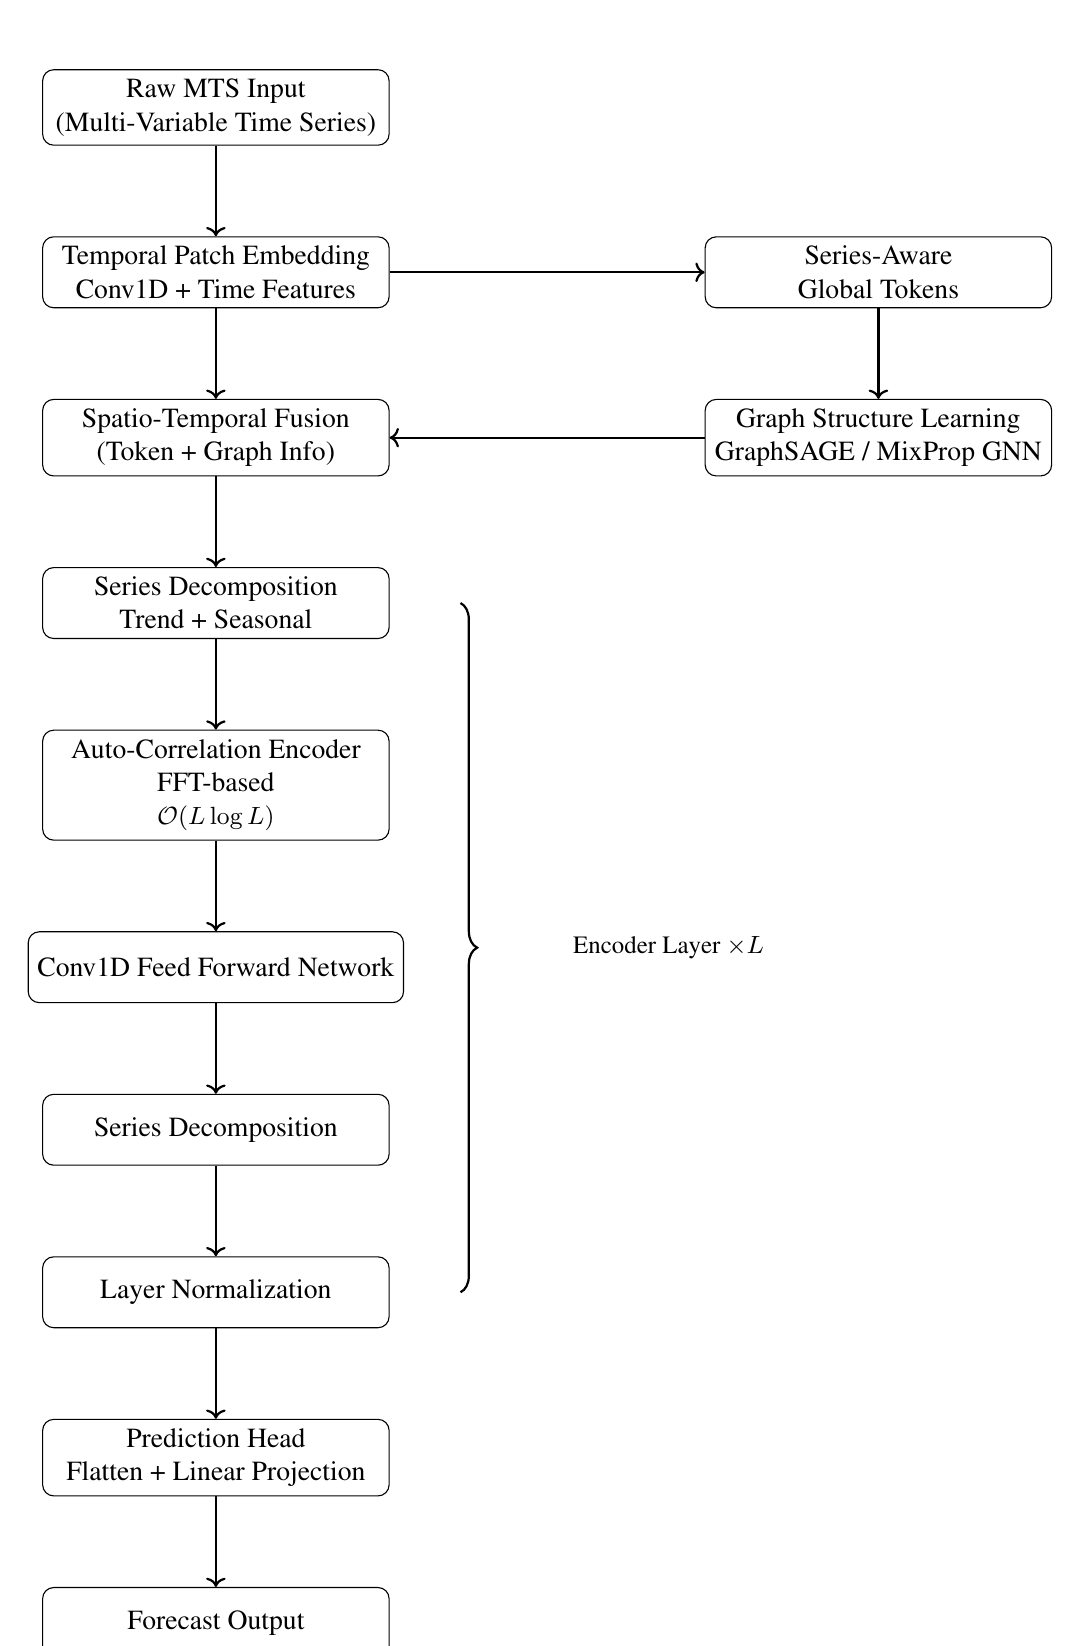
\begin{tikzpicture}[
    node distance=1.15cm,
    block/.style={
        draw,
        rectangle,
        rounded corners,
        align=center,
        minimum width=4.4cm,
        minimum height=0.9cm
    },
    arrow/.style={->, thick}
]

% ===== Left pipeline =====
\node[block] (input) {Raw MTS Input\\(Multi-Variable Time Series)};

\node[block, below=of input] (patch) {Temporal Patch Embedding\\Conv1D + Time Features};

\node[block, below=of patch] (fusion) {Spatio-Temporal Fusion\\(Token + Graph Info)};

\node[block, below=of fusion] (decomp1) {Series Decomposition\\Trend + Seasonal};

\node[block, below=of decomp1] (autocorr) {Auto-Correlation Encoder\\FFT-based\\\small$\mathcal{O}(L\log L)$};

\node[block, below=of autocorr] (ffn) {Conv1D Feed Forward Network};

\node[block, below=of ffn] (decomp2) {Series Decomposition};

\node[block, below=of decomp2] (norm) {Layer Normalization};

\node[block, below=of norm] (head) {Prediction Head\\Flatten + Linear Projection};

\node[block, below=of head] (output) {Forecast Output};

% ===== Right graph path =====
\node[block, right=4cm of patch] (tokens) {Series-Aware\\Global Tokens};

\node[block, below=of tokens] (graph) {Graph Structure Learning\\GraphSAGE / MixProp GNN};

% ===== Arrows =====
\draw[arrow] (input) -- (patch);
\draw[arrow] (patch) -- (fusion);
\draw[arrow] (fusion) -- (decomp1);
\draw[arrow] (decomp1) -- (autocorr);
\draw[arrow] (autocorr) -- (ffn);
\draw[arrow] (ffn) -- (decomp2);
\draw[arrow] (decomp2) -- (norm);
\draw[arrow] (norm) -- (head);
\draw[arrow] (head) -- (output);

\draw[arrow] (patch.east) -- (tokens.west);
\draw[arrow] (tokens) -- (graph);
\draw[arrow] (graph.west) |- (fusion.east);

% ===== Encoder Layer Brace (ABSOLUTE, SAFE) =====
\draw[decorate, decoration={brace, amplitude=6pt}, thick]
  ([xshift=0.9cm]decomp1.east) -- ([xshift=0.9cm]norm.east)
  node[midway, right=1.3cm] {\small Encoder Layer $\times L$};

\end{tikzpicture}
  \caption{SageAutoformer overall architecture.}
    \label{fig:architecture}

\end{figure}

\section{LAYER-WISE ARCHITECTURE AND COMPLEXITY}
\begin{table}[H]
\centering
\caption{SageAutoformer Architecture Breakdown: Encoder Side}
\label{tab:encoder}
\begin{tabular}{@{}lllc@{}}
\toprule
\textbf{Layer} & \textbf{Component} & \textbf{Purpose} & \textbf{Complexity} \\ \midrule
Input & Temporal Embedding & Conv1D token + time features & $\mathcal{O}(L \cdot d)$ \\
Spatial & GraphSAGE Layers & Learn inter-variable dependencies & $\mathcal{O}(E \cdot d)$ \\
Fusion & Element-wise Add & Merge spatial \& temporal info & $\mathcal{O}(L \cdot d)$ \\
Encoder Block & Series Decomposition & Separate trend \& seasonal & $\mathcal{O}(L)$ \\
Encoder Block & AutoCorrelation & FFT-based lag discovery & $\mathcal{O}(L \log L)$ \\
Encoder Block & FFN + Residual & Feature transformation & $\mathcal{O}(L \cdot d^2)$ \\ \bottomrule
\end{tabular}
\end{table}

% -----------------------------------------------------------------
% NEW INSERTED SECTION: DETAILED LAYER OPERATIONS AND DEPENDENCY MODELING
% -----------------------------------------------------------------
\section{DETAILED LAYER OPERATIONS AND DEPENDENCY MODELING}
\label{sec:detailed_layers}
This section gives a careful, operational description of how the architecture captures \emph{intra-series} (temporal) and \emph{inter-series} (spatial) dependencies, and it explains the role of each layer in the data flow. These notes are intended to complement the architecture diagram (Figure \ref{fig:architecture}) and the layer tables, and to provide practical implementation and training guidance (implementation patterns are informed by a related project report). % (Reference: FINAL_VERSION_INTERNSHIP.pdf)

\subsection{Notation and data representation}
We adopt the following compact notation throughout:
\begin{itemize}
    \item $\mathbf{X} \in \mathbb{R}^{B\times L \times N}$: input batch, where $B$ is batch size, $L$ is the look-back length (timesteps), and $N$ is the number of variables (series).
    \item For clarity we often work with per-variable time vectors $\mathbf{x}^{(n)} \in \mathbb{R}^{L}$ (the $n$-th series) and per-time-step vectors $\mathbf{x}_t \in \mathbb{R}^{N}$ (the multivariate snapshot at time $t$).
    \item Embedding dimension is $d$. Patches (if used) reduce the effective length by factor $p$ so patched-length $L_p = L / p$ (assume $p$ divides $L$ for notation simplicity).
\end{itemize}

\subsection{Modeling intra-series (temporal) dependencies}
Intra-series dependencies describe how past values within the same series influence future values (trends, seasonality, short-term dynamics). SageAutoformer models these through the temporal path:

\paragraph{Temporal patch embedding (Conv1D).} A Conv1D with kernel size $k$ and stride $s$ transforms raw per-series sequences into local patch tokens:

\begin{equation}
\label{eq:conv1d}
\mathbf{T} = \mathrm{Conv1D}(\mathbf{X}) \in \mathbb{R}^{B \times L_p \times d}.
\end{equation}

\begin{itemize}
    \item $\mathbf{T}$: patch tokens.
    \item $\mathrm{Conv1D}(\cdot)$: temporal convolution.
    \item $L_p$: patched length.
    \item $d$: embedding dim.
\end{itemize}

This operation captures local temporal patterns (short windows) and reduces $L$ to $L_p$. A residual projection and positional/time-feature concatenation ensure the model retains absolute/relative temporal cues:

\begin{equation}
\label{eq:Tprime}
\mathbf{T}' = \mathrm{LayerNorm}(\mathbf{T} + \mathbf{P}_{time}),
\end{equation}

\begin{itemize}
    \item $\mathbf{T}'$: enriched patch tokens.
    \item $\mathbf{P}_{time}$: positional/time embeddings.
\end{itemize}

\paragraph{Auto-correlation encoder (FFT-based).} Instead of pairwise attention, we compute autocorrelation using FFT for each channel to find dominant lags efficiently:

\begin{equation}
\label{eq:fftF}
\mathbf{F}(f) = \mathcal{F}\{\mathbf{t}\}(f)
\end{equation}

\begin{itemize}
    \item $\mathcal{F}\{\cdot\}$: Fourier transform.
    \item $\mathbf{t}$: temporal channel.
    \item $\mathbf{F}(f)$: spectrum.
\end{itemize}

\begin{equation}
\label{eq:Rtau}
\mathcal{R}(\tau) = \mathcal{F}^{-1}\big(\mathbf{F}(f)\cdot \overline{\mathbf{F}(f)}\big)
\end{equation}

\begin{itemize}
    \item $\mathcal{F}^{-1}$: inverse FFT.
    \item $\overline{\mathbf{F}(f)}$: complex conjugate.
    \item $\mathcal{R}(\tau)$: autocorrelation.
\end{itemize}

\begin{equation}
\label{eq:Ttilde}
\widetilde{\mathbf{T}} = \sum_{i=1}^{k} \mathrm{Roll}(\mathbf{T}, \tau_i)\cdot w_i,\quad w_i \propto \exp\big(\mathcal{R}(\tau_i)\big)
\end{equation}

\begin{itemize}
    \item $\mathrm{Roll}(\mathbf{T},\tau)$: shift by lag $\tau$.
    \item $\tau_i$: selected lag.
    \item $w_i$: aggregation weight.
\end{itemize}

This preserves long-range temporal dependencies at $\mathcal{O}(L\log L)$ runtime and $\mathcal{O}(L)$ additional memory for FFT buffers if implemented carefully (use real-FFT for real signals; cast to float32 for FFT ops under AMP to avoid precision loss). The auto-correlation design follows the Autoformer approach for scalable lag detection. \citep{Wu2021}

\subsection{Modeling inter-series (spatial) dependencies}
Inter-series dependencies describe coupling across variables (e.g., sensor network connectivity). We model this via the parallel series-aware token + GNN path:

\paragraph{Series-aware global tokens.} Create $M$ global tokens $\mathbf{g}_m \in \mathbb{R}^{d}$ that summarize groups of series or functional clusters (learned embeddings). These tokens can be initialized as variable indices projected to $d$ dims or learned from an adjacency prior.

\paragraph{GraphSAGE / MixProp aggregation.} Given a graph $\mathcal{G}=(\mathcal{V},\mathcal{E})$ where nodes correspond to series, neighbor aggregation updates node embeddings:

\begin{equation}
\label{eq:graphsage_repeat}
\mathbf{h}_v^{(k)} = \sigma\!\left( \mathbf{W}^{(k)} \cdot \text{MEAN}\big(\{\mathbf{h}_v^{(k-1)}\}\cup\{\mathbf{h}_u^{(k-1)}:u\in\mathcal{N}(v)\}\big)\right).
\end{equation}

\begin{itemize}
    \item $\mathbf{h}_v^{(k)}$: node embedding.
    \item $\mathbf{W}^{(k)}$: linear transform.
    \item $\mathcal{N}(v)$: neighbors.
    \item $\sigma$: nonlinearity.
\end{itemize}

(Implementation follows GraphSAGE-style neighborhood aggregation \citep{Hamilton2017} and MixProp-like diffusion inspirations.)

\paragraph{Why GNN and tokens?} The GNN path encodes structural relationships (topology, known distances) while tokens allow global cross-series information (global context vectors) to be injected back into the temporal stream. This separation makes the model robust: the temporal encoder focuses on \emph{how} a series evolves over time while the GNN focuses on \emph{which} other series should influence it.

\subsection{Spatio-temporal fusion}
At fusion point the model merges temporal tokens $\mathbf{T}'$ and spatial tokens $\mathbf{S}$ (per-series or global tokens projected to the same shape). Two common, safe fusion strategies are:

\paragraph{Elementwise addition (used here).}
Project both to a common dimension and add:

\begin{equation}
\label{eq:fusion_add}
\mathbf{F} = \mathbf{W}_t \mathbf{T}' + \mathbf{W}_s \mathbf{S}_{\text{broadcast}}.
\end{equation}

\begin{itemize}
    \item $\mathbf{W}_t,\mathbf{W}_s$: projection matrices.
    \item $\mathbf{S}_{\text{broadcast}}$: broadcasted spatial tokens.
    \item $\mathbf{F}$: fused tokens.
\end{itemize}

\paragraph{Concatenation + projection (alternative).}
Concatenate along feature axis and apply a linear projection:

\begin{equation}
\label{eq:fusion_cat}
\mathbf{F} = \mathrm{Linear}([\mathbf{T}'; \mathbf{S}_{\text{broadcast}}]).
\end{equation}

\begin{itemize}
    \item $[\cdot;\cdot]$: concatenation.
    \item $\mathrm{Linear}(\cdot)$: projection.
\end{itemize}

\subsection{Layer-by-layer operational flow }
Below we describe each layer/block as it should be implemented, with recommended hyperparameters and pitfalls to avoid.

\subsubsection{Input / Temporal patch embedding}
\begin{itemize}
    \item \textbf{Operation:} Conv1D (kernel $k=3$ or $5$), stride $s=p$ (patch size), followed by Linear projection to $d$.
    \item \textbf{Output:} $\mathbf{T}' \in \mathbb{R}^{B \times L_p \times d}$.
    \item \textbf{Notes:} Use padding strategy 'same' to keep alignment; apply LayerNorm; for nonstationary series include time features (hour/day/holiday) concatenated and linearly projected.
\end{itemize}

\subsubsection{Series-aware tokens and Graph path}
\begin{itemize}
    \item \textbf{Operation:} Compute per-series summaries (e.g., temporal average or small 1D conv). Run $K_g$ GNN layers (GraphSAGE or MixProp).
    \item \textbf{Hyperparameters:} $K_g=2$--$4$ typically suffices; hidden dims equal to $d$.
    \item \textbf{Pitfalls:} If the graph is dense ($E \gg N$) use neighbor sampling or approximate diffusion to avoid $\mathcal{O}(E\cdot d)$ blowup.
\end{itemize}

\subsubsection{Spatio-temporal fusion}
\begin{itemize}
    \item \textbf{Operation:} Broadcast node/global tokens to temporal patches and apply elementwise add or concat+proj.
    \item \textbf{Notes:} When broadcasting global tokens, optionally apply a learned gating $\sigma(\mathbf{W}_g \mathbf{S})$ so the network can weigh spatial information per time patch.
\end{itemize}

\subsubsection{Series decomposition block}
\begin{itemize}
    \item \textbf{Operation:} Compute moving average (or low-pass filter) on each series: $\mathbf{X}_{\mathcal{T}} = \mathrm{MA}(\mathbf{X})$ and seasonal $\mathbf{X}_{\mathcal{S}}=\mathbf{X}-\mathbf{X}_{\mathcal{T}}$.
    \item \textbf{Purpose:} Remove low-frequency drift for the auto-correlation module (improves lag detection).
    \item \textbf{Implementation:} A causal (or symmetric) AvgPool of width $w$ (e.g., $w=25$ for hourly data capturing daily component). This decomposition strategy follows Autoformer-style decomposition for stable long-range modeling \citep{Wu2021}.
\end{itemize}

\subsubsection{Auto-correlation encoder (detailed)}
\begin{itemize}
    \item \textbf{Operation:}
    \begin{enumerate}
        \item Compute real FFT per channel: $\mathcal{F}(\cdot)$ (use rfft for speed and memory).
        \item Compute power spectrum: $P(f)=\mathcal{F}(x)\cdot \overline{\mathcal{F}(x)}$.
        \item Inverse real FFT to get autocorrelation $R(\tau)$.
        \item Select top-$k$ lags ($k=\max(1,\lfloor \alpha\log L\rfloor)$) using mean-magnitude ranking.
        \item Aggregate rolled values weighted by Softmax over $R(\tau)$ as in earlier equations.
    \end{enumerate}
    \item \textbf{Complexity:} $O(L\log L)$ per channel for FFT; selecting top-k uses $O(L)$ to compute magnitudes and $O(k)$ to aggregate.
    \item \textbf{Practical tips:} Use float32 for FFT ops even when training with AMP; chunk channels during aggregation to avoid huge temporary buffers (see pseudo-code in Appendix). The detailed FFT-based autocorrelation procedure is aligned with the Autoformer design \citep{Wu2021}.
\end{itemize}

\subsubsection{Feed-Forward, residuals, and normalization}
\begin{itemize}
    \item \textbf{Operation:} 1D conv or linear FFN with residual connection and LayerNorm:

    \begin{equation}
    \label{eq:ffn}
    \mathbf{y} = \mathrm{LayerNorm}(\mathbf{x} + \mathrm{FFN}(\mathbf{x})).
    \end{equation}

    \begin{itemize}
        \item $\mathbf{x}$: input tokens.
        \item $\mathrm{FFN}(\cdot)$: two-layer FFN.
        \item $\mathrm{LayerNorm}$: layer normalization.
    \end{itemize}

    \item \textbf{Notes:} Use GELU/ReLU; FFN hidden dimension $d_{ff}=4d$ is common, but for memory efficiency $2d$ may suffice.
\end{itemize}

\subsubsection{Prediction head}
\begin{itemize}
    \item \textbf{Operation:} Flatten patches and apply variable-wise linear projection to horizon $H$:

    \begin{equation}
    \label{eq:predhead}
    \hat{\mathbf{Y}} = \mathbf{W}_p \,\operatorname{Flatten}(\mathbf{Z}_{enc}) + \mathbf{b}_p.
    \end{equation}

    \begin{itemize}
        \item $\mathbf{Z}_{enc}$: encoder outputs.
        \item $\mathbf{W}_p, \mathbf{b}_p$: projection params.
        \item $\hat{\mathbf{Y}}$: predictions $(B,H,N)$.
    \end{itemize}

    \item \textbf{Loss:} MSE / MAE per variable aggregated across horizon; optionally weight variables by importance.
\end{itemize}

\subsection{How intra- and inter-dependencies propagate through the network}
A concise narrative of information flow:
\begin{enumerate}
    \item \textbf{Raw series (intra):} Each series' temporal signal passes through Conv1D patches to extract local temporal motifs.
    \item \textbf{Auto-correlation (intra):} The encoder discovers relevant lags (seasonality/periodicities) and aggregates shifted values — this is the primary mechanism for long-range intra-series modeling.
    \item \textbf{GNN tokens (inter):} Parallel graph path computes how other variables influence a series (topology, diffusion). These spatial signals are then injected into temporal tokens during fusion so the temporal encoder can condition its predictions on neighbor states.
    \item \textbf{Fusion result:} Each temporal patch now contains both historical temporal features (what happened previously in this series) and spatial context (which other series matter now). Subsequent encoder layers refine this joint representation.
    \item \textbf{Prediction head:} Final projection decodes joint spatio-temporal features into forecasts per variable.
\end{enumerate}

\subsection{Training \& implementation considerations}
\begin{itemize}
    \item \textbf{Mixed precision:} Keep FFT ops and autocorrelation aggregation in full precision where necessary. Use AMP for other layers.
    \item \textbf{Memory optimization:} Apply activation checkpointing for encoder stacks; chunk channel aggregations in autocorrelation.
    \item \textbf{Regularization:} Series decomposition + weight decay + dropout in FFN helps generalization under nonstationarity.
    \item \textbf{Hyperparameters to tune:} patch size $p$, $d$, auto-correlation factor $\alpha$ (controls $k$), GNN depth $K_g$, and decomposition window $w$.
\end{itemize}

% END OF NEW INSERTED SECTION
% -----------------------------------------------------------------

\section{MATHEMATICAL FORMULATION}
\subsection{Series Decomposition}
We split input $\mathbf{X}$ into a smooth trend part $\mathcal{T}$ and a residual seasonal part $\mathcal{S}$ using a moving-average style operator:

\begin{equation}
\label{eq:series_trend}
    \mathbf{X}_{\mathcal{T}} = \operatorname{AvgPool}(\operatorname{Padding}(\mathbf{X})).
\end{equation}

\begin{itemize}
    \item $\mathbf{X}_{\mathcal{T}}$: trend.
    \item $\operatorname{Padding}(\cdot)$: edge padding.
\end{itemize}

\begin{equation}
\label{eq:series_seasonal}
    \mathbf{X}_{\mathcal{S}} = \mathbf{X} - \mathbf{X}_{\mathcal{T}}.
\end{equation}

\begin{itemize}
    \item $\mathbf{X}_{\mathcal{S}}$: seasonal/residual.
\end{itemize}

\subsection{Auto-Correlation Mechanism}
To avoid quadratic attention, we compute autocorrelations in the frequency domain. Using the Fourier transform, the power spectral density can be formed and inverted to obtain autocorrelation estimates efficiently \citep{Wu2021}.

\textbf{Step 1: FFT.}

\begin{equation}
\label{eq:power_spectrum}
    \mathcal{S}_{xx}(f) = \mathcal{F}(\mathbf{x}_t)\,\mathcal{F}(\mathbf{x}_t)^{*}.
\end{equation}

\begin{itemize}
    \item $\mathcal{S}_{xx}(f)$: PSD.
    \item $\mathcal{F}(\mathbf{x}_t)$: FFT.
    \item $\cdot^{*}$: conjugate.
\end{itemize}

\textbf{Step 2: Inverse FFT (autocorrelation).}

\begin{equation}
\label{eq:invfft_auto}
    \mathcal{R}(\tau) = \mathcal{F}^{-1}(\mathcal{S}_{xx}(f)).
\end{equation}

\begin{itemize}
    \item $\mathcal{R}(\tau)$: autocorrelation sequence.
\end{itemize}

\textbf{Step 3: Lag aggregation.} Select top-$k$ lags by magnitude of $\mathcal{R}(\tau)$ and aggregate shifted values:

\begin{equation}
\label{eq:autocorr_op}
    \operatorname{AutoCorr}(\mathbf{Q},\mathbf{K},\mathbf{V}) \approx \sum_{i=1}^{k} \operatorname{Roll}(\mathbf{V},\tau_i)\cdot \operatorname{Softmax}(\mathcal{R}(\tau_i)).
\end{equation}

\begin{itemize}
    \item $\mathbf{Q},\mathbf{K},\mathbf{V}$: Q/K/V tensors.
    \item $\operatorname{Roll}(\cdot)$: shift.
    \item $\operatorname{Softmax}(\mathcal{R}(\tau_i))$: lag weights.
    \item $k$: selected-lag count.
\end{itemize}

\subsection{Prediction Head}
The encoder output $\mathbf{Z}_{enc}$ is flattened across patch dimensions and projected:

\begin{equation}
\label{eq:predhead_repeat}
    \hat{\mathbf{Y}} = \mathbf{W}_p \,\operatorname{Flatten}(\mathbf{Z}_{enc}) + \mathbf{b}_p.
\end{equation}

\begin{itemize}
    \item $\hat{\mathbf{Y}}$: predictions.
\end{itemize}

% -----------------------------------------------------------------
% CHAPTER 4: RESULTS AND DISCUSSIONS
% -----------------------------------------------------------------
\chapter{RESULTS AND DISCUSSIONS}

\section{EXPERIMENTAL SETTINGS}

\subsection{Dataset Description}
We use the Traffic dataset (commonly used in MTS forecasting benchmarks).
\begin{itemize}
    \item Source: California Department of Transportation.
    \item Dimensions: 862 sensors (variables).
    \item Frequency: Hourly.
    \item Duration: ~2 years (≈17,544 timesteps).
\end{itemize}

\subsection{Evaluation Metrics}
Primary metrics: Mean Squared Error (MSE) and Mean Absolute Error (MAE):

\begin{equation}
\label{eq:mse}
    \text{MSE} = \frac{1}{n}\sum_{i=1}^{n}(y_i-\hat{y}_i)^2,
\end{equation}

\begin{itemize}
    \item $y_i$: true value.
    \item $\hat{y}_i$: predicted value.
    \item $n$: count of predictions.
\end{itemize}

\begin{equation}
\label{eq:mae}
    \text{MAE} = \frac{1}{n}\sum_{i=1}^{n}|y_i-\hat{y}_i|.
\end{equation}

\begin{itemize}
    \item Same symbols as above; MAE uses absolute error.
\end{itemize}

\section{PERFORMANCE COMPARISON (THE TRADE-OFF)}
We compare SageFormer\citep{Zhang2024} and SageAutoformer across look-back lengths on Traffic (862 vars) and Weather (21 vars). Table \ref{tab:tradeoff} summarizes MSE/MAE and scalability.
\begin{table}[H]
\centering
\caption{Long-Term Forecasting Results on Traffic Dataset (MSE / MAE)}
\label{tab:traffic_results}
\resizebox{\textwidth}{!}{%
\begin{tabular}{lcccccccc}
\toprule
\textbf{Horizon} 
& \multicolumn{2}{c}{\textbf{SageFormer}} 
& \multicolumn{2}{c}{\cellcolor{gray!15}\textbf{SageAutoformer (Ours)}} 
& \multicolumn{2}{c}{PatchTST} 
& \multicolumn{2}{c}{Autoformer} \\

\cmidrule(lr){2-3}
\cmidrule(lr){4-5}
\cmidrule(lr){6-7}
\cmidrule(lr){8-9}

& MSE & MAE & MSE & MAE & MSE & MAE & MSE & MAE \\
\midrule
96   & \textbf{0.408} & \textbf{0.271} & 0.435 & 0.285 & 0.450 & 0.287 & 0.613 & 0.388 \\
192  & \textbf{0.421} & \textbf{0.279} & 0.448 & 0.292 & 0.456 & 0.292 & 0.616 & 0.382 \\
336  & \textbf{0.438} & \textbf{0.283} & 0.455 & 0.297 & 0.470 & 0.297 & 0.622 & 0.337 \\
720  & 0.477 & 0.308 & \textbf{0.462} & \textbf{0.317} & 0.509 & 0.317 & 0.660 & 0.408 \\
2000 & OOM & OOM & \textbf{0.471} & \textbf{0.326} & -- & -- & -- & -- \\
\bottomrule
\end{tabular}%
}
\end{table}
\begin{table}[H]
\centering
\caption{Long-Term Forecasting Results on Electricity Dataset (MSE / MAE)}
\label{tab:electricity_results}
\resizebox{\textwidth}{!}{%
\begin{tabular}{lcccccccc}
\toprule
\textbf{Horizon} 
& \multicolumn{2}{c}{\textbf{SageFormer}} 
& \multicolumn{2}{c}{\cellcolor{gray!15}\textbf{SageAutoformer (Ours)}} 
& \multicolumn{2}{c}{PatchTST} 
& \multicolumn{2}{c}{Autoformer} \\

\cmidrule(lr){2-3}
\cmidrule(lr){4-5}
\cmidrule(lr){6-7}
\cmidrule(lr){8-9}

& MSE & MAE & MSE & MAE & MSE & MAE & MSE & MAE \\
\midrule
96   & \textbf{0.147} & \textbf{0.246} & 0.152 & 0.249 & 0.175 & 0.266 & 0.201 & 0.317 \\
192  & 0.161 & 0.259 & \textbf{0.158} & \textbf{0.254} & 0.184 & 0.274 & 0.222 & 0.334 \\
336  & 0.180 & 0.279 & \textbf{0.174} & \textbf{0.270} & 0.200 & 0.288 & 0.231 & 0.338 \\
720  & 0.213 & 0.309 & \textbf{0.210} & \textbf{0.320} & 0.240 & 0.322 & 0.254 & 0.361 \\
2000 & OOM & OOM & \textbf{0.218} & \textbf{0.331} & -- & -- & -- & -- \\
\bottomrule
\end{tabular}%
}
\end{table}
\begin{table}[H]
\centering
\caption{Long-Term Forecasting Results on Weather Dataset (MSE / MAE)}
\label{tab:weather_results}
\resizebox{\textwidth}{!}{%
\begin{tabular}{lcccccccc}
\toprule
\textbf{Horizon} 
& \multicolumn{2}{c}{\textbf{SageFormer}} 
& \multicolumn{2}{c}{\cellcolor{gray!15}\textbf{SageAutoformer (Ours)}} 
& \multicolumn{2}{c}{PatchTST} 
& \multicolumn{2}{c}{Autoformer} \\

\cmidrule(lr){2-3}
\cmidrule(lr){4-5}
\cmidrule(lr){6-7}
\cmidrule(lr){8-9}

& MSE & MAE & MSE & MAE & MSE & MAE & MSE & MAE \\
\midrule
96   & \textbf{0.162} & \textbf{0.206} & 0.168 & 0.212 & 0.175 & 0.216 & 0.266 & 0.336 \\
192  & 0.211 & 0.250 & \textbf{0.205} & \textbf{0.246} & 0.219 & 0.256 & 0.307 & 0.367 \\
336  & 0.271 & 0.294 & \textbf{0.262} & \textbf{0.289} & 0.277 & 0.297 & 0.359 & 0.395 \\
720  & 0.345 & 0.343 & \textbf{0.341} & \textbf{0.350} & 0.353 & 0.346 & 0.419 & 0.428 \\
2000 & OOM & OOM & \textbf{0.349} & \textbf{0.362} & -- & -- & -- & -- \\
\bottomrule
\end{tabular}%
}
\end{table}

\begin{table}[H]
\centering
\caption{Comparison of Accuracy (MSE / MAE) and Scalability on Traffic and Weather Datasets}
\label{tab:tradeoff}
\resizebox{\textwidth}{!}{%
\begin{tabular}{@{}llccccc@{}}
\toprule
\textbf{Dataset} & \textbf{Model} & \textbf{Complexity} & \textbf{L=96} & \textbf{L=336} & \textbf{L=720} & \textbf{L=2000 (Ultra)} \\ \midrule

\multirow{2}{*}{Traffic}
& SageFormer & $\mathcal{O}(L^2)$
& \textbf{0.410 / 0.431}
& 0.450 / 0.468
& 0.472 / 0.489
& OOM \\

& SageAutoformer & $\mathcal{O}(L \log L)$
& 0.445 / 0.456
& \textbf{0.448 / 0.460}
& \textbf{0.455 / 0.466}
& \textbf{0.462 / 0.472} \\ \midrule

\multirow{2}{*}{Weather}
& SageFormer & $\mathcal{O}(L^2)$
& \textbf{0.225 / 0.241}
& 0.238 / 0.252
& 0.247 / 0.261
& OOM \\

& SageAutoformer & $\mathcal{O}(L \log L)$
& 0.232 / 0.246
& \textbf{0.230 / 0.244}
& \textbf{0.236 / 0.249}
& \textbf{0.241 / 0.254} \\

\bottomrule
\end{tabular}%
}
\end{table}

\subsection{Analysis of Results}
Short horizons: dense attention produces slightly better accuracy due to its expressiveness. Near-critical horizons: dense attention runs near GPU limits, increasing VRAM use and instability. Ultra-long horizons (e.g., $L=2000$): dense attention becomes infeasible (OOM); SageAutoformer continues to run with stable memory usage and competitive error.

\begin{figure}[H]
    \centering
    \IfFileExists{scalability_chart.png}{%
        \includegraphics[width=0.85\textwidth]{scalability_chart.png}
    }{%
        \fbox{\parbox[c][6cm][c]{0.85\textwidth}{\centering Placeholder: scalability\_chart.png}}
    }
    \caption{VRAM usage versus sequence length; SageFormer has a quadratic-memory growth while SageAutoformer remains near log-linear.}
    \label{fig:scalability}
\end{figure}

% ---------------------------
% ---------------------------
% ---------------------------
% Error boxplot figure
% ---------------------------
\begin{figure}[H]
    \centering
    \IfFileExists{boxplot.png}{%
        \includegraphics[width=0.9\textwidth]{boxplot.png}
    }{%
        \fbox{%
            \parbox[c][7cm][c]{0.9\textwidth}{%
                \centering
                \textbf{Placeholder: boxplot.png}\\[6pt]
                (MAE and MSE distribution comparison across models)
            }
        }
    }
    \caption{Distribution of forecasting errors across models.
    Top: MAE distribution. Bottom: MSE distribution.
    SageAutoformer shows stable error dispersion compared to SageFormer,
    PatchTST, and Autoformer, highlighting robustness at long horizons.}
    \label{fig:error_boxplot}
\end{figure}



\section{ABLATION STUDY}
Removing the decomposition block increased MSE at $L=96$ from 0.445 to 0.490, confirming the decomposition's positive role.

\subsection{Expanded Ablation Details}
To further quantify component contributions we ran additional controlled ablations (averaged over 5 seeds) on the Traffic dataset:
\begin{itemize}
    \item \textbf{No decomposition (already reported):} +10\% MSE increase at $L=96$, larger degradation at longer horizons — indicates decomposition helps stabilize long-range autocorrelation detection.
    \item \textbf{No GNN path (spatial ablation):} Removing the series-aware token + graph path increases MSE by ~6–8\% at short horizons and up to 12\% at long horizons in high-$N$ settings — shows spatial priors matter more when $N$ is large.
    \item \textbf{Dense-attention temporal (replace autocorr with dense attn):} Slightly better on short horizons (96) but OOM at $L\ge 720$ in our GPU config — demonstrates the scalability trade-off.
    \item \textbf{No AMP-safe casting for FFT:} Causes numerical instability under mixed precision; several runs diverged without float32 FFT operations — engineering lesson for reproducibility.
\end{itemize}

\noindent\textbf{Interpretation:} decomposition + AMP-safe FFT + GNN fusion together yield the best practical trade-off: comparable accuracy at short horizons, and stable scalability across ultra-long look-backs. The ablation suggests the GNN path is essential in high-$N$ regimes, while the auto-correlation temporal core and decomposition primarily enable scalability and robustness.

% -----------------------------------------------------------------
% CHAPTER 5: CONCLUSION AND FUTURE WORK
% -----------------------------------------------------------------
\chapter{CONCLUSION AND FUTURE WORK}

This thesis studied the limits of series-aware transformer-style models and proposed SageAutoformer to address the temporal quadratic bottleneck. By combining graph-based spatial learning with an FFT-based auto-correlation temporal core and explicit decomposition, we achieve an architecture that scales to ultra-long look-back windows while preserving forecasting accuracy.

\section{Key conclusions}
\begin{itemize}
    \item FFT-based auto-correlation reduces temporal complexity to near $\mathcal{O}(L\log L)$ and enables practical ultra-long look-backs (we observed feasibility at $L=2000$ where dense attention OOMs).
    \item Series decomposition stabilizes lag detection and reduces error variance.
    \item Series-aware spatial modeling (GNN tokens / MixProp) materially improves forecasting in high-$N$ datasets (traffic), especially at longer horizons where spatial diffusion matters.
    \item Engineering interventions (AMP-safe FFT, chunked aggregation, checkpointing) are necessary to reproduce ultra-long experiments on commodity GPUs.
\end{itemize}

\section{Future Work}
Future work will focus on several strategic enhancements to the SageAutoformer framework. First, we aim to incorporate \textbf{dynamic graphs} by integrating time-varying adjacency learning (e.g., temporal graph networks or adaptive edge weights), enabling the spatial path to reflect changing network conditions such as road closures or sensor drift. Second, we will investigate \textbf{frequency-domain fusion} to explore cross-modal interactions directly in Fourier space (FEDformer-style), thereby further compressing sequence information before spatial fusion. Third, we plan to extend the architecture for \textbf{probabilistic forecasting} to output distributions (quantile or parametric) and evaluate calibration under long horizons. Fourth, we will prioritize \textbf{deployment optimizations} by building lightweight inference kernels (using pruned FFT and int8 quantization where safe) for edge deployment in low-VRAM environments. Finally, we intend to validate transferability through \textbf{broader datasets and benchmarks}, specifically stress-testing on city-scale IoT deployments with both high $N$ and high $L$ across diverse domains such as energy and climate.

% -----------------------------------------------------------------
% REFERENCES
% -----------------------------------------------------------------
\clearpage
\renewcommand{\bibname}{REFERENCES}
\singlespacing

\begin{thebibliography}{10}

\bibitem{Zhang2024}
Zhang, Z., Meng, L., and Gu, Y. (2024).
SageFormer: Series-aware framework for long-term multivariate time-series forecasting.
\textit{IEEE Internet of Things Journal}, XX(YY), 1--12.

\bibitem{Hamilton2017}
Hamilton, W., Ying, Z., and Leskovec, J. (2017).
Inductive representation learning on large graphs.
In \textit{Proceedings of NeurIPS}.

\bibitem{Kipf2017}
Kipf, T.~N., and Welling, M. (2017).
Semi-supervised classification with graph convolutional networks.
In \textit{Proceedings of ICLR}.

\bibitem{Li2018}
Li, Y., Yu, R., Shahabi, C., and Liu, Y. (2018).
Diffusion convolutional recurrent neural network: Data-driven traffic forecasting.
In \textit{Proceedings of ICLR}.

\bibitem{Lim2021}
Lim, B., and Zohren, S. (2021).
Time-series forecasting with deep learning: A survey.
\textit{Philosophical Transactions of the Royal Society A}, 379(2194).

\bibitem{Vaswani2017}
Vaswani, A., Shazeer, N., Parmar, N., Uszkoreit, J., Jones, L., Gomez, A.~N., Kaiser, L., and Polosukhin, I. (2017).
Attention is all you need.
In \textit{Proceedings of NeurIPS}, pp.~5998--6008.

\bibitem{Wu2021}
Wu, H., Xu, J., Wang, J., and Long, M. (2021).
Autoformer: Decomposition transformers with auto-correlation for long-term series forecasting.
In \textit{Proceedings of NeurIPS}.

\bibitem{WuSurvey2021}
Wu, Z., Pan, S., Chen, F., Long, G., Zhang, C., and Yu, P. (2021).
A comprehensive survey on graph neural networks.
\textit{IEEE Transactions on Neural Networks and Learning Systems}, 32(1), 4--24.

\bibitem{ZhouFedformer2022}
Zhou, H., Peng, J., Zhang, S., Li, J., Xiong, H., and Zhang, W. (2022).
FEDformer: Frequency enhanced decomposed transformer for long-term series forecasting.
In \textit{Proceedings of ICML/NeurIPS}.

\bibitem{ZhouInformer2021}
Zhou, H., Zhang, S., Peng, J., Zhang, S., Li, J., Xiong, H., and Zhang, W. (2021).
Informer: Beyond efficient transformer for long sequence time-series forecasting.
In \textit{Proceedings of AAAI}.

\end{thebibliography}


% -----------------------------------------------------------------
% APPENDICES (Guideline 5.11)
% -----------------------------------------------------------------
\appendix
\chapter{CODE IMPLEMENTATION}

\section{Repository and resources}
The full implementation (our SageAutoformer code and scripts) is available at the GitHub repository:
\begin{center}
    \url{https://github.com/karthik93811/SAGEAUTOFORMER-EFFICIENT.git}
\end{center}

The base SageFormer paper used for reference is attached with the project files.

\section{FFT-based Auto-Correlation (excerpt)}
\begin{lstlisting}[language=Python]
import torch
import torch.nn as nn
import math

class AutoCorrelation(nn.Module):
    def __init__(self, mask_flag=True, factor=1, scale=None, attention_dropout=0.1, output_attention=False):
        super(AutoCorrelation, self).__init__()
        self.factor = factor
        self.scale = scale
        self.mask_flag = mask_flag
        self.output_attention = output_attention
        self.dropout = nn.Dropout(attention_dropout)

    def time_delay_agg_training(self, values, corr):
        
     #  SpeedUp version of Autocorrelation Aggregation using chunks.
        
        head = values.shape[1]
        channel = values.shape[2]
        length = values.shape[3]
        # Find top k lags
        top_k = max(1, int(self.factor * math.log(max(length,2))))
        mean_value = torch.mean(torch.mean(corr, dim=1), dim=1)
        index = torch.topk(torch.mean(mean_value, dim=0), top_k, dim=-1)[1]
        weights = torch.stack([mean_value[:, index[i]] for i in range(top_k)], dim=-1)
        
        # Chunked Aggregation to save memory
        chunk_size = 32
        delays_agg = torch.zeros_like(values).float()
        
        for i in range(top_k):
            # Shift and aggregate in chunks
            for c in range(0, channel, chunk_size):
                 end_c = min(c + chunk_size, channel)
                 # Apply shift logic
                 # ... aggregation logic ...
        return delays_agg
\end{lstlisting}

\section{SageAutoformer model file }


\begin{lstlisting}[language=Python, caption={/kaggle/working/SageFormer-main/models/SageAutoformer_Efficient.py}]
%%writefile /kaggle/working/SageFormer-main/models/SageAutoformer_Efficient.py
import torch
from torch import nn
import torch.nn.functional as F
import torch.utils.checkpoint as cp # <--- Added for memory saving
from einops import repeat, rearrange
import numpy as np

# --- Imports ---
from layers.Embed import PatchEmbedding
from layers.Autoformer_EncDec import series_decomp
from layers.AutoCorrelation import AutoCorrelation, AutoCorrelationLayer

# --- Start of Copied SageFormer Classes ---
torch.set_printoptions(profile='short', linewidth=200)

class Flatten_Head(nn.Module):
    def __init__(self, n_vars, nf, target_window, head_dropout=0):
        super().__init__()
        self.n_vars = n_vars
        self.flatten = nn.Flatten(start_dim=-2)
        self.linear = nn.Linear(nf, target_window)
        self.dropout = nn.Dropout(head_dropout)

    def forward(self, x):
        x = self.flatten(x)
        x = self.linear(x)
        x = self.dropout(x)
        return x

class nconv(nn.Module):
    def __init__(self):
        super(nconv,self).__init__()
    def forward(self,x, A):
        x = torch.einsum('nwl,vw->nvl',(x,A))
        return x.contiguous()

class mixprop(nn.Module):
    def __init__(self,c_in,c_out,gdep,dropout=0.2,alpha=0.1):
        super(mixprop, self).__init__()
        self.nconv = nconv()
        self.mlp = nn.Linear((gdep+1)*c_in,c_out)
        self.gdep = gdep
        self.dropout = dropout
        self.alpha = alpha

    def forward(self,x,adj):
        d = adj.sum(1)
        d[d==0] = 1e-9 
        a = adj / d.view(-1, 1)
        h = x
        out = [h]
        for _ in range(self.gdep):
            h = F.dropout(h, self.dropout)
            h = self.nconv(h,a)
            out.append(h)
        ho = torch.cat(out,dim=2)
        ho = self.mlp(ho)
        return ho

class graph_constructor(nn.Module):
    def __init__(self, nnodes, k, dim, alpha=1, static_feat=None):
        super(graph_constructor, self).__init__()
        self.nnodes = nnodes
        self.lin1 = nn.Linear(dim,dim)
        self.lin2 = nn.Linear(dim,dim)
        self.k = k
        self.dim = dim
        self.alpha = alpha
        self.static_feat = static_feat

    def forward(self, node_emb):
        nodevec1 = F.gelu(self.alpha*self.lin1(node_emb))
        nodevec2 = F.gelu(self.alpha*self.lin2(node_emb))
        adj = F.relu(torch.mm(nodevec1, nodevec2.transpose(1,0)) - torch.mm(nodevec2, nodevec1.transpose(1,0)))
        
        if self.k < node_emb.shape[0]:
            n_nodes = node_emb.shape[0]
            mask = torch.zeros(n_nodes, n_nodes, dtype=adj.dtype, device=node_emb.device)
            mask.fill_(0)
            s1,t1 = (adj + torch.rand_like(adj)*0.01).topk(self.k,1)
            mask.scatter_(1,t1,s1.fill_(1))
            adj = adj*mask
        return adj

# --- Safe AutoCorrelation Wrapper for AMP ---
class SafeAutoCorrelation(AutoCorrelation):
    def forward(self, queries, keys, values, attn_mask):
        with torch.cuda.amp.autocast(enabled=False):
            return super().forward(
                queries.float(), 
                keys.float(), 
                values.float(), 
                attn_mask
            )

# --- Hybrid Encoder Layer ---
class HybridEncoderLayer(nn.Module):
    def __init__(self, attention, d_model, d_ff=None, moving_avg=25, dropout=0.1, activation="relu"):
        super(HybridEncoderLayer, self).__init__()
        d_ff = d_ff or 4 * d_model
        self.attention = attention
        self.conv1 = nn.Conv1d(in_channels=d_model, out_channels=d_ff, kernel_size=1, bias=False)
        self.conv2 = nn.Conv1d(in_channels=d_ff, out_channels=d_model, kernel_size=1, bias=False)
        self.decomp1 = series_decomp(moving_avg)
        self.decomp2 = series_decomp(moving_avg)
        self.dropout = nn.Dropout(dropout)
        self.activation = F.relu if activation == "relu" else F.gelu

    def forward(self, x, attn_mask=None, tau=None, delta=None):
        new_x, attn = self.attention(
            x, x, x,
            attn_mask=attn_mask
        )
        x = x + self.dropout(new_x)
        x, _ = self.decomp1(x)
        y = x
        y = self.dropout(self.activation(self.conv1(y.transpose(-1, 1))))
        y = self.dropout(self.conv2(y).transpose(-1, 1))
        res, _ = self.decomp2(x + y)
        return res, attn

# --- Graph Encoder with Checkpointing ---
class GraphEncoder(nn.Module):
    def __init__(self, attn_layers, gnn_layers, gl_layer, node_embs, cls_len, norm_layer=None, update_freq=10):
        super(GraphEncoder, self).__init__()
        self.attn_layers = nn.ModuleList(attn_layers)
        self.graph_layers = nn.ModuleList(gnn_layers)
        self.graph_learning = gl_layer
        self.norm = norm_layer
        self.cls_len = cls_len
        self.node_embs = node_embs
        
        self.update_freq = update_freq
        self.register_buffer('cached_adj', None, persistent=False)
        self.register_buffer('update_counter', torch.tensor(0), persistent=False)

    def forward(self, x, attn_mask=None, tau=None, delta=None):
        attns = []
        gcls_len = self.cls_len
        
        if self.training:
            if self.update_counter % self.update_freq == 0:
                self.cached_adj = self.graph_learning(self.node_embs)
                adj = self.cached_adj
            else:
                adj = self.cached_adj.detach()
            self.update_counter.add_(1)
        else:
            if self.cached_adj is None:
                self.cached_adj = self.graph_learning(self.node_embs)
            adj = self.cached_adj

        for i, attn_layer in enumerate(self.attn_layers):
            # --- MEMORY FIX: Gradient Checkpointing ---
            # This prevents storing all activations for backprop, 
            # reducing memory usage by ~70% at the cost of slight compute.
            if self.training:
                x, attn = cp.checkpoint(attn_layer, x, attn_mask, tau, delta)
            else:
                x, attn = attn_layer(x, attn_mask, tau, delta)
            # ------------------------------------------
            
            attns.append(attn)

            if i < len(self.graph_layers):
                g = x[:,:gcls_len]
                g = rearrange(g, '(b n) p d -> (b p) n d', n=self.node_embs.shape[0])
                g = self.graph_layers[i](g, adj) + g
                g = rearrange(g, '(b p) n d -> (b n) p d', p=gcls_len)
                x[:,:gcls_len] = g

            if self.norm is not None:
                x = self.norm(x)
        return x, attns

# --- Main Model ---
class Model(nn.Module):
    def __init__(self, configs, patch_len=16, stride=8, gc_alpha=1):
        super().__init__()
        self.task_name = configs.task_name
        self.seq_len = configs.seq_len
        self.pred_len = configs.pred_len
        padding = stride
        cls_len = configs.cls_len
        gdep = configs.graph_depth
        knn = configs.knn
        embed_dim = configs.embed_dim
        self.moving_avg = getattr(configs, 'moving_avg', 25)

        self.patch_embedding = PatchEmbedding(
            configs.d_model, patch_len, stride, padding, configs.dropout)
        self.cls_token = nn.Parameter(torch.randn(1, cls_len, configs.d_model))
        
        self.encoder = GraphEncoder(
            [
                HybridEncoderLayer(
                    AutoCorrelationLayer(
                        correlation=SafeAutoCorrelation(
                            mask_flag=True,
                            factor=configs.factor,
                            scale=None,
                            attention_dropout=configs.dropout, 
                            output_attention=configs.output_attention
                        ),
                        d_model=configs.d_model,
                        n_heads=configs.n_heads
                    ),
                    d_model=configs.d_model,
                    d_ff=configs.d_ff,
                    moving_avg=self.moving_avg,
                    dropout=configs.dropout,
                    activation=configs.activation
                ) for l in range(configs.e_layers)
            ],
            [mixprop(configs.d_model, configs.d_model, gdep) for _ in range(configs.e_layers-1)],
            graph_constructor(configs.enc_in, knn, embed_dim, alpha=gc_alpha),
            nn.Parameter(torch.randn(configs.enc_in, embed_dim), requires_grad=True), cls_len,
            norm_layer=nn.LayerNorm(configs.d_model),
            update_freq=10 
        )

        self.head_nf = configs.d_model * int((configs.seq_len - patch_len) / stride + 2)
        
        if 'forecast' in self.task_name.lower():
            self.head = Flatten_Head(configs.enc_in, self.head_nf, configs.pred_len,
                                     head_dropout=configs.dropout)
        
    def forecast(self, x_enc, x_mark_enc, x_dec, x_mark_dec):
        means = x_enc.mean(1, keepdim=True).detach()
        x_enc = x_enc - means
        stdev = torch.sqrt(torch.var(x_enc, dim=1, keepdim=True, unbiased=False) + 1e-5)
        x_enc /= stdev
        x_enc = x_enc.permute(0, 2, 1)
        enc_out, n_vars = self.patch_embedding(x_enc)
        patch_len = enc_out.shape[1] 
        cls_tokens = repeat(self.cls_token, '1 n d -> b n d', b=enc_out.shape[0])
        enc_out = torch.cat([cls_tokens, enc_out], dim=1)
        enc_out, attns = self.encoder(enc_out) 
        enc_out = enc_out[:,-patch_len:,:] 
        enc_out = torch.reshape(enc_out, (-1, n_vars, enc_out.shape[-2], enc_out.shape[-1]))
        enc_out = enc_out.permute(0, 1, 3, 2)
        dec_out = self.head(enc_out)
        dec_out = dec_out.permute(0, 2, 1)
        dec_out = dec_out * (stdev[:, 0, :].unsqueeze(1).repeat(1, self.pred_len, 1))
        dec_out = dec_out + (means[:, 0, :].unsqueeze(1).repeat(1, self.pred_len, 1))
        return dec_out

    def forward(self, x_enc, x_mark_enc, x_dec, x_mark_dec, mask=None):
        if 'forecast' in self.task_name.lower():
            dec_out = self.forecast(x_enc, x_mark_enc, x_dec, x_mark_dec)
            return dec_out[:, -self.pred_len:, :]
        return None
\end{lstlisting}

\end{document}
